\documentclass[aspectratio=1610]{beamer}
\usepackage{tikz, xcolor, amsmath, minted}
\definecolor{webgreen}{rgb}{.3, .7, .3}
\color{webgreen}
%\setbeamercolor{structure}{fg=webgreen} 
%\color{webgreen}
\begin{document}
\begin{frame}
\title{Data Structures and Algorithms}
\subtitle{Singly Linked List}
\author{Shiv S. Dayal}
\titlepage
\end{frame}

\begin{frame}[fragile]
\frametitle{Basics of a singly linked list}
\begin{itemize}
\item Let us consider a piece of singly linked list data structure.
\begin{minted}[frame=lines]{c}
typedef struct linked_list {
  int data;
  struct linked_list *next;
}ll;
\end{minted}
\item Here \texttt{data} is integer but it can be any other data type
also for example, a character or float or pointer or string or
union or structures or any other conceivable data type.
\item The second element is a mandatory poiter capable of pointing to
structures of the same type of which it is a member.
\item Such structures are called \textit{self-referential} structures.
\end{itemize}
\end{frame}

\begin{frame}
\frametitle{Basic operations}
Basic operations on a linked list are:
\begin{itemize}
\item Insertion,
\item Deletion,
\item Search, and
\item Count
\end{itemize}
Insertion is tricky because it can be at the beginning, in
between and at the end. Although, it can be abstracted like
\texttt{insert(element, head, position);} and behind the
scenes we can implement different logic depending on the case.

Head pointer of linked list is typically written as \texttt{head}
or \texttt{p}. We will use the name as \texttt{head}.

Let us try to see these operations graphically.
\end{frame}

\begin{frame}
\frametitle{Insertion at beginning}
\textbf{Case I.} When list in empty.
\begin{center}
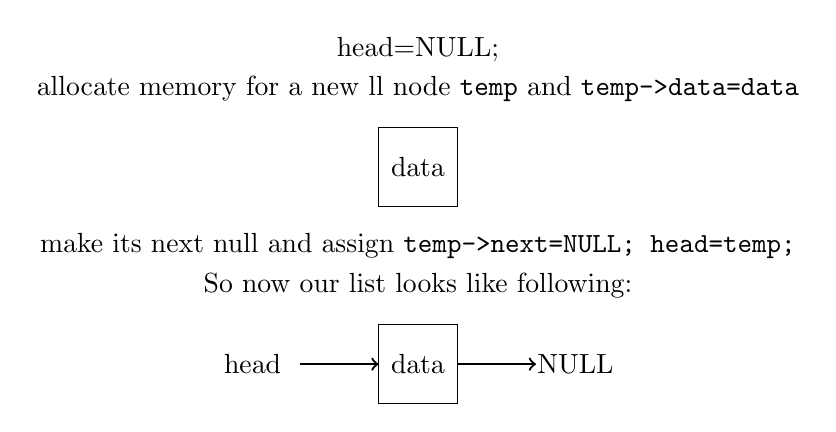
\begin{tikzpicture}
\draw(0,7) node{head=NULL;};
\draw (0,6.5) node{allocate memory for a new ll node \texttt{temp} and \texttt{temp->data=data}};
\draw (-0.5,5) rectangle (.5,6);
\draw (0,5.5) node{data};
\draw (0,4.5) node{make its next null and assign \texttt{temp->next=NULL; head=temp;}};
\draw (0,4) node{So now our list looks like following:};
\draw (-.5,2.5) rectangle (.5,3.5);
\draw[->, thick] (-1.5,3) -- (-0.5,3);
\draw (0,3) node{data};
\draw (-2.1, 3) node{head};
\draw[->, thick] (.5,3) -- (1.5,3);
\draw (2,3) node{NULL};
\end{tikzpicture}
\end{center}
\end{frame}
\begin{frame}
\textbf{Case II.} When the list is not empty.
\begin{center}
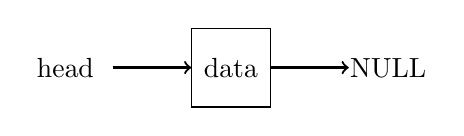
\begin{tikzpicture}
\draw (-.5,6.5) rectangle (.5,7.5);
\draw[->, thick] (-1.5,7) -- (-0.5,7);
\draw (0,7) node{data};
\draw (-2.1, 7) node{head};
\draw[->, thick] (.5,7) -- (1.5,7);
\draw (2,7) node{NULL};
\end{tikzpicture}
\end{center}
We allocate a new node \texttt{temp} and assign \texttt{temp->next=head;temp->data=data1;}
then list would look something like following:
\begin{center}
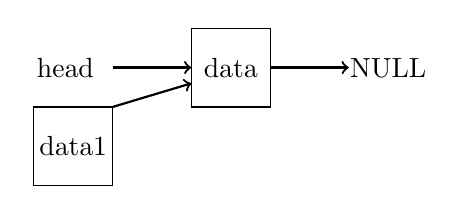
\begin{tikzpicture}
\draw (-.5,2.5) rectangle (.5,3.5);
\draw[->, thick] (-1.5,3) -- (-0.5,3);
\draw (0,3) node{data};
\draw (-2.1, 3) node{head};
\draw[->, thick] (.5,3) -- (1.5,3);
\draw (2,3) node{NULL};
\draw (-2.5,1.5) rectangle (-1.5,2.5);
\draw (-2,2) node{data1};
\draw[->, thick] (-1.5,2.5) -- (-0.5,2.8);
\end{tikzpicture}
\end{center}
Now, we can move \texttt{head} to point to \texttt{temp1} by saying
\texttt{head=temp1;} then our list would look like fowllowing:
\end{frame}
\begin{frame}[fragile]
\begin{center}
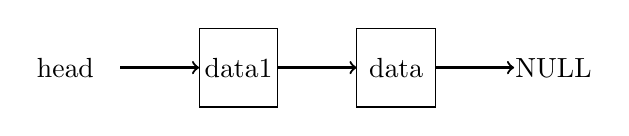
\begin{tikzpicture}
\draw (-.5,6.5) rectangle (.5,7.5);
\draw[->, thick] (-1.5,7) -- (-0.5,7);
\draw (0,7) node{data};
\draw[->, thick] (.5,7) -- (1.5,7);
\draw (2,7) node{NULL};
\draw (-2.5,6.5) rectangle (-1.5,7.5);
\draw (-2,7) node{data1};
\draw[->, thick] (-3.5,7) -- (-2.5,7);
\draw (-4.2,7) node {head};
\end{tikzpicture}
\end{center}
The code for this operation is given below:
\begin{minted}[linenos]{c}
void add_at_beg(ll** head)
{
  ll *temp;
  int i;

  temp = (ll*)malloc(sizeof(ll));

  printf("Enter an integer to be added at beginning\n");
  scanf("%d", &i);

  temp->next = *head;
  *head = temp;
  (*head)->data = i;
}
\end{minted}
\end{frame}
\begin{frame}
\frametitle{Complexity of insertion at beginning}
Let us say cost for operations of line no. 6, 8, 9, 11, 12 and 13 are
$c_1, c_2, c_3, c_4, c_5 \text{ and } c_6$. Then total cost is
$\sum_{i=1}^6 c_i$ which is constant, say $K$, so $K$ is $MO(1)$ where
for any $M>K$ the order $O(1)$ will provide an upper bound.

\end{frame}

\begin{frame}
\frametitle{Insertion in between two nodes}
\textbf{Insertion at some position}
If position is 0 then we can simply call \texttt{add\_at\_beg} described
earlier. If not then clearly list is not empty. So we need to move forward
in linked list using \texttt{head=head->next;} till we reach our desired
position or \texttt{head->next} becomes \texttt{NULL}.

If we reach our position we allocate memory for a temporary node and
manipulate pointers to put this new node in between.

Supposed we do it for position 1 with starting node being at 0. Then
considering our previous linked list. Let us say we put data x in this
new node.
\begin{center}
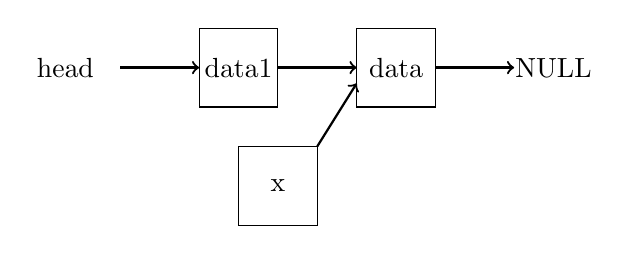
\begin{tikzpicture}
\draw (-.5,6.5) rectangle (.5,7.5);
\draw[->, thick] (-1.5,7) -- (-0.5,7);
\draw (0,7) node{data};
\draw[->, thick] (.5,7) -- (1.5,7);
\draw (2,7) node{NULL};
\draw (-2.5,6.5) rectangle (-1.5,7.5);
\draw (-2,7) node{data1};
\draw[->, thick] (-3.5,7) -- (-2.5,7);
\draw (-4.2,7) node {head};
\draw (-2,5) rectangle (-1,6);
\draw (-1.5,5.5) node{x};
\draw[->, thick] (-1,6) -- (-.5, 6.8);
\end{tikzpicture}
\end{center}
Now we simply point \texttt{data1->next} which is actually
\texttt{head} because we did \texttt{head=head->next;} to arrive
here. We say \texttt{head->next=temp;} where \texttt{temp} is
this allocated node.
\end{frame}

\begin{frame}[fragile]
So now our list would look like following:
\begin{center}
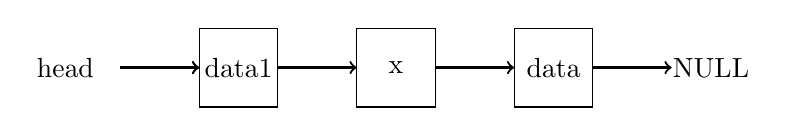
\begin{tikzpicture}
\draw (-.5,6.5) rectangle (.5,7.5);
\draw[->, thick] (-1.5,7) -- (-0.5,7);
\draw (0,7) node{x};
\draw[->, thick] (.5,7) -- (1.5,7);
\draw (4,7) node{NULL};
\draw (-2.5,6.5) rectangle (-1.5,7.5);
\draw (-2,7) node{data1};
\draw[->, thick] (-3.5,7) -- (-2.5,7);
\draw (-4.2,7) node {head};
\draw (1.5,6.5) rectangle (2.5,7.5);
\draw (2,7) node{data};
\draw[->, thick] (-3.5,7) -- (-2.5,7);
\draw[->, thick] (2.5,7) -- (3.5,7);
\end{tikzpicture}
\end{center}
\begin{minted}{c}
void add_in_bet(ll* head)
{
  ll *temp;
  int i = 0, j = 0;
  int position = 0;

  temp = (ll*)malloc(sizeof(ll));

  printf("Enter position at which the number is to be added.\n");
  scanf("%d", &position);

  if(position == 0)
    return add_at_beg(&head);

  printf("Enter an integer to be added in between.\n");
  scanf("%d", &i);
\end{minted}
\end{frame}
\begin{frame}[fragile]
\begin{minted}{c}
  while(head->next != NULL) {
    ++j;
    if(j == position) {
      temp->next = head->next;
      head->next = temp;
      temp->data = i;
      break;
    }
    head = head->next;
  }
}
\end{minted}

\vspace*{0.5cm}
\textbf{Complexity analysis}
\vspace*{0.5cm}

Most of cost of operations is constant what depends on variable position
is \texttt{++j} and \texttt{head=head->next;}. Now suppose there are
\texttt{n} elements then worst case is $O(n)$ because we can always have a
large constant $M$.
\end{frame}
\end{document}

